\section{Intensity Interferometry (II) with IACT arrays}
R. Hanbury Brown and Robert Q. Twiss (HBT) carried out the first experiments demonstrating the possibility of measuring angular diameter of stars using Intensity Interferometry (II) in optical wavelengths \citep{HBT56}. Subsequently, they also pioneered the theoretical background of II and conducted laboratory experiments \citep{brown1957interferometry,brown1958interferometry},thereby further consolidating II as an alternative method, besides the already established Michelson Interferometry, to measure stars. Further, HBT also successfully installed the Narrabri Stellar Intensity Interferometer \textcolor{blue}{during the 1960s-70s and successfully used it to measure the angular diameters of bright stars in the spectral range $\mathrm{O5f}\ -\ \mathrm{F8}$ using visible wavelengths} signals \citep{brown1974intensity}. \\\textcolor{blue}
{However, the available speed and sensitivity of electronics in the 1970s was not favourable for more extensive and larger scale measurement projects using II.}

\textcolor{blue}{Subsequently, during the opening decades of the current century, proposals to use the Imaging Atmospheric Cherenkov Telescope (IACT) facilities for carrying out Stellar Intensity Interferometry (SII) observations were put forth \citep{LeBohec2006, nunez2010stellar, nunez2012high, Dravins2013}. Such observations, it was suggested, could be carried out during bright moon-lit nights during which $\gamma$-ray observations using upper atmospheric Cherenkov showers were not feasible. This idea had the potential of enhancing the scientific output of the existing facilities like VERITAS, MAGIC and HESS. Subsequent SII obserations at these facilities providing the proof of concept have been published \citep{abeysekara2020demonstration, Abe2024MAGIC, Zmija2023}. }

\textcolor{blue}{In the remaining part of this section, we present a brief conceptual procedure of how an array of Cherenkov telescopes is used to carry out II observations and generate Signal-to-Noise Ratio (SNR) from these observations.}

\subsection{The signal for II}\label{sec:signal}
As a simple example, let us consider the pair of IACTs at MAGIC. Let us imagine that the two telescopes, namely, MAGIC-I and MAGIC-II are pointed to a star. \textcolor{red}{My comment: As our model has 4 hypothetical IACTs and we are not taking any specific properties of the MAGIC telescopes into the calculations or into the model, it would be better to avoid using the specific names of MAGIC facility.This portion can be easily rewritten without the mention of MAGIC.}Let them simultaneously measure the intensity of radiation $I_1(t)$ a  and $I_2(t)$ respectively. These signals from the respective detectors are cross-correlated and averaged over time and yield the \textcolor{blue}{second order ($n=2$) correlation of these intensities as}  \citep{acciari2020optical, dravins2013optical}
\begin{equation}
	g^{(2)}= \frac{\left\langle I_1(t) \cdot I_2(t + \tau) \right\rangle}{\langle I_1(t) \rangle \cdot \langle I_2(t) \rangle} 
	\label{eqn:HBT}
\end{equation}
where $\tau$ is the time delay between the telescopes. \st{If the light source is chaotic and randomly polarized,}\textcolor{blue}{For a spatially coherent and randomly polarized light, eq.(\ref{eqn:HBT}) reduces to the Siegert relation \citep{acciari2020optical}}
\begin{equation}
	g^{(2)} = 1 + \frac{\Delta f}{\Delta \nu} \abs{V_{12}}^2
	\label{eqn:HBT2}
\end{equation}
where, $\Delta f$ is the electronic bandwidth \textcolor{blue}{of the photon detectors (that measure the intensities and typically lie in range $\sim 100 {\mathrm {MHz}}$)} and $\Delta {\mathrm {\nu}}$ is the optical bandwidth \textcolor{blue}{of radiation over which the intensities are measured}\footnote{\textcolor{blue}{Typically, filters with bandwidths in the range $\Delta \lambda \sim 20 nm - 50 nm$ corresponding to $\Delta \nu \sim 10^{15}$ Hz are used.} . In eq.(\ref{eqn:HBT2}), $V_{12}$, referred to as the complex visibility fuction, is the Fourier transform of the source brightness distribution and is given by
\begin{equation}
\vert V_{12} \vert = 2 \frac{J_1(\pi \ d \ {\theta}/{\lambda})}{\pi\  d \ {\theta}/{\lambda}}
\label{eqn:absvisib}
\end{equation}
with $d$, $\theta$ and $\lambda$ being the baseline, the angular diameter of the star and the optical wavelength of the filter used in observation.
It is obvious from eq(\ref{eqn:absvisib}) that $\vert V_{12} \vert$ carries the information of the angular diameter of the star.} However, the phase information is lost \st{due to the involvement of the absolute value of $V_{12}$}\textcolor{blue}{as we measure the absolute value $\vert V_{12} \vert$}. In observational astronomy, the correlation is often expressed in terms of the normalized contrast, given by:
\begin{equation}
	c = \frac{\left\langle \left( I_1(t) - \left\langle I_1 \right\rangle \right) \cdot \left( I_2(t + \tau) - \left\langle I_2 \right\rangle \right) \right\rangle}{\langle I_1(t) \rangle \cdot \langle I_2(t) \rangle} = g^{(2)} - 1
\end{equation}
where, $\left\langle I_1 \right\rangle$ and $\left\langle I_2 \right\rangle$ are the mean intensity from two telescopes.

\textcolor{red}{Insert text (may be one more paragraph) to extend the expression for $g^{(2)}$ or $c$ to include the signals from more number of baselines. This will be important because we are considering a set of 4 IACTs in our model and therefore 6 baselines.}


\subsection{The Signal-to-Noise Ratio for II}
\begin{figure}
	\centering
	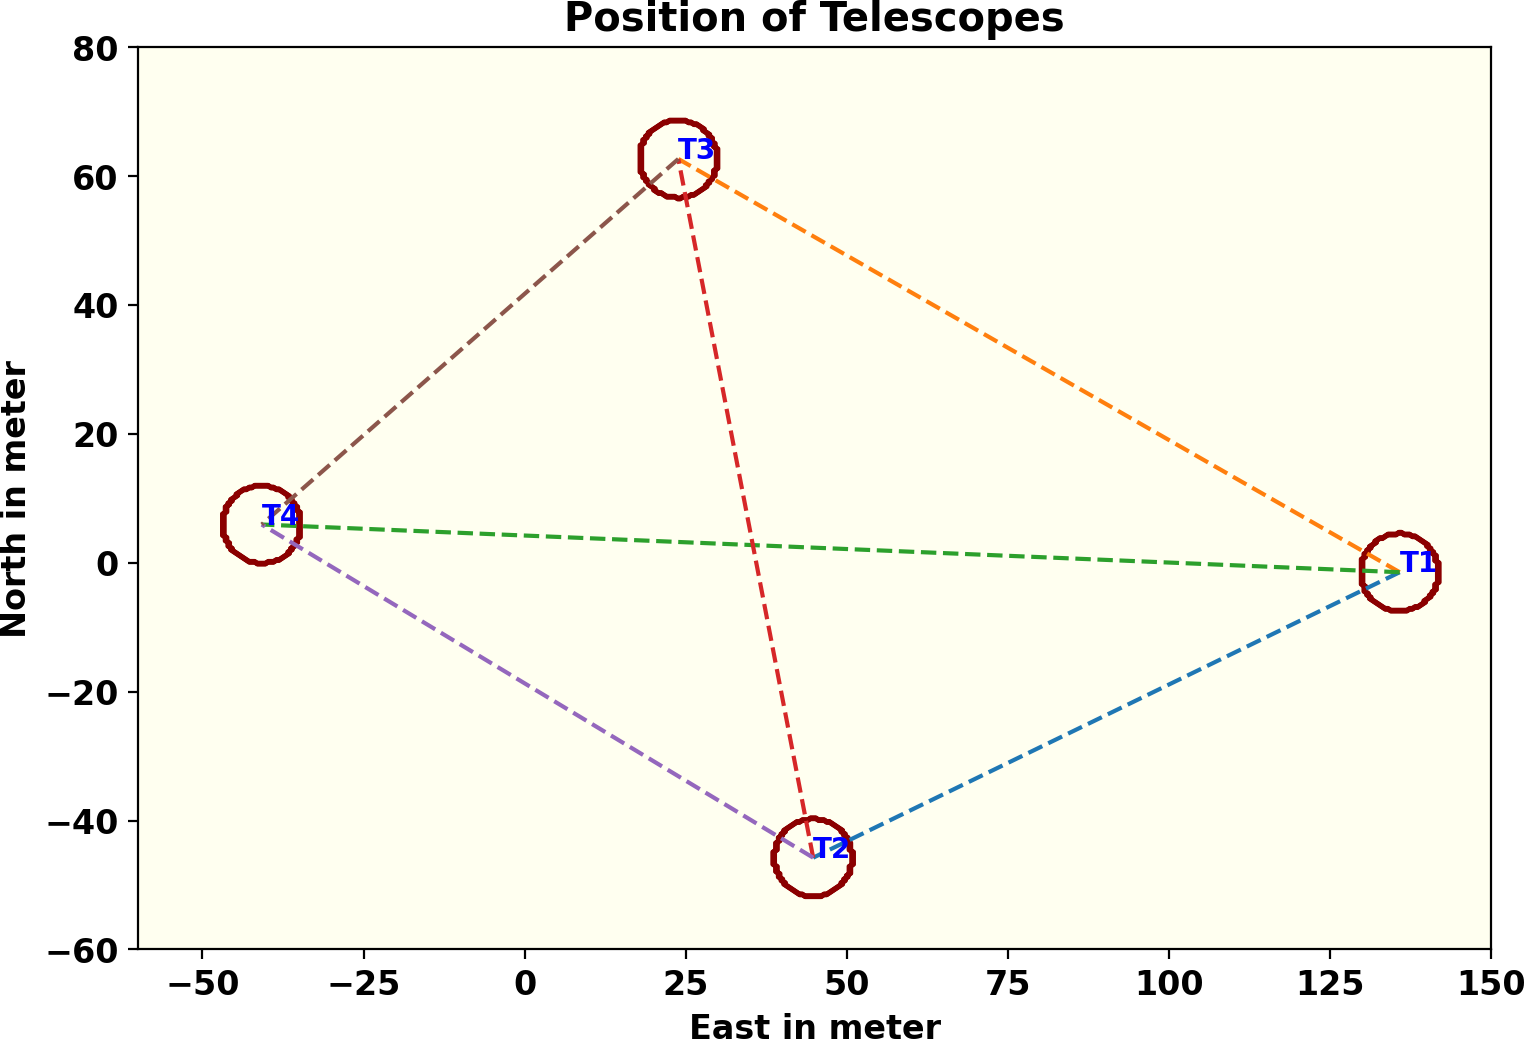
\includegraphics[width=\linewidth]{fig/telescope.png}
	\caption{The telescope configuration with similar properties each used to simulate the signal for II.}
	\label{fig:teles}
\end{figure}
\begin{figure}
	\centering
	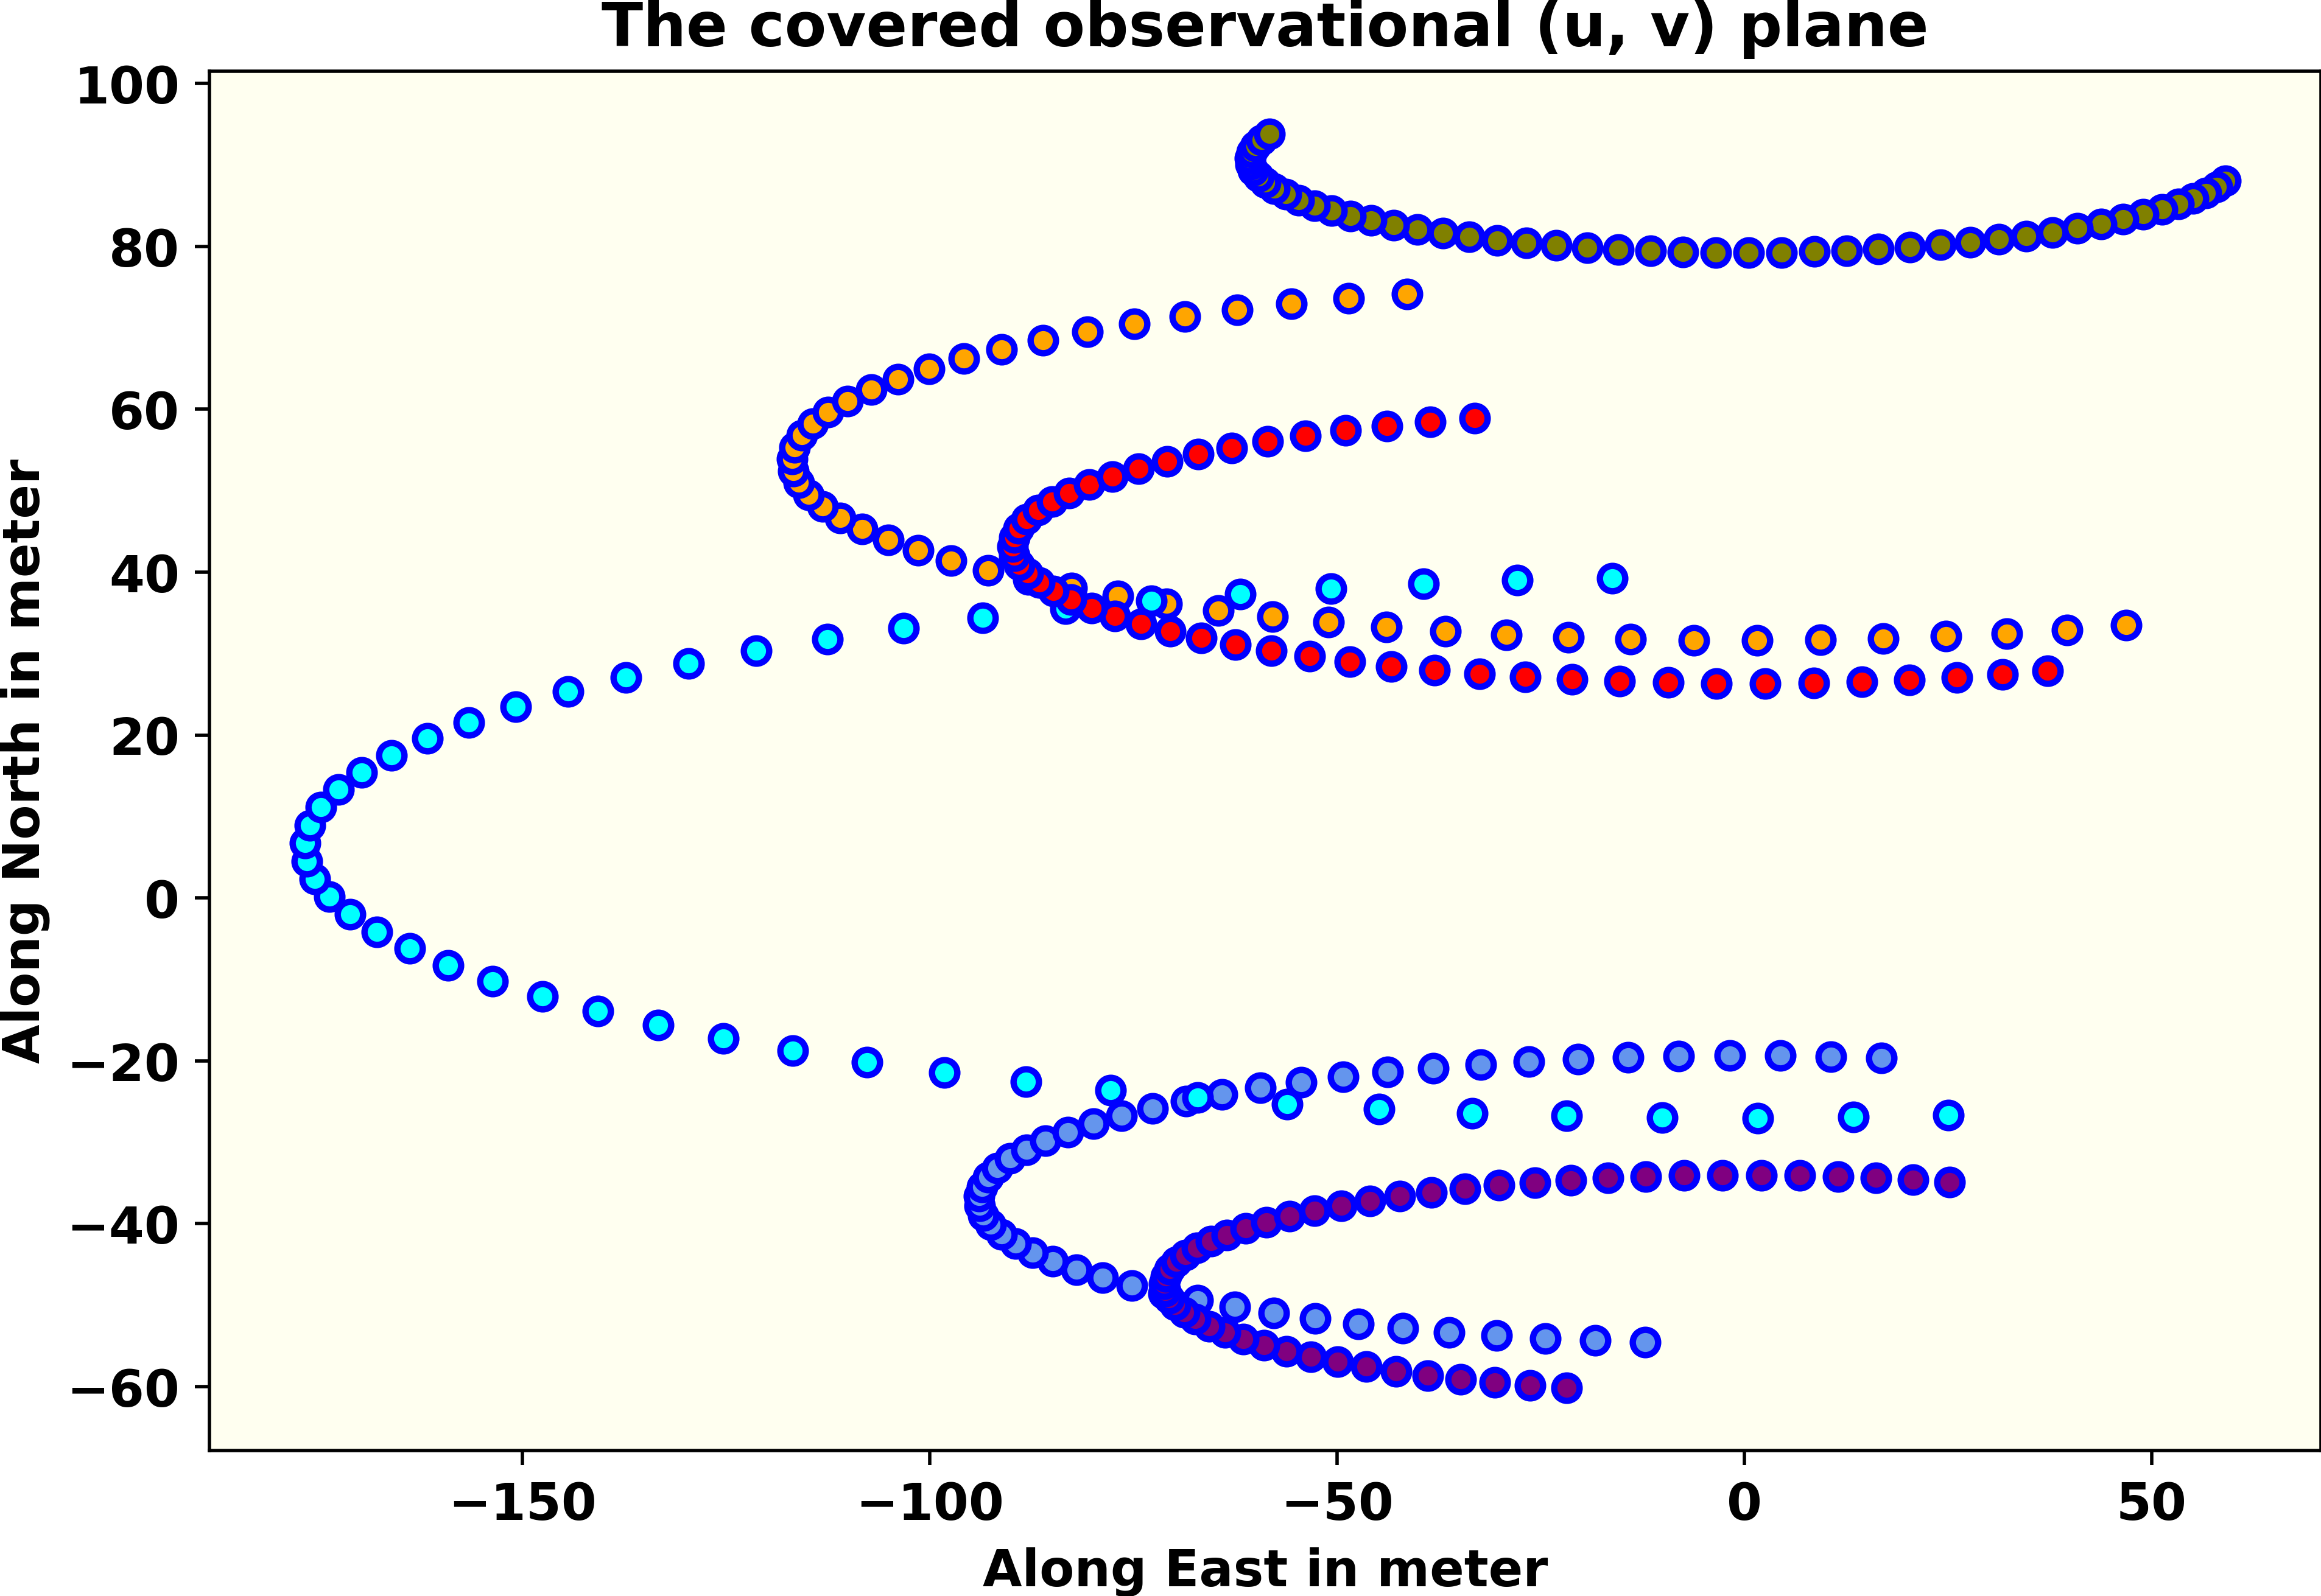
\includegraphics[width=\linewidth]{fig/baseline.png}
	\caption{The tracking of baselines with four telescopes arranged in fig.~\ref{fig:teles} for one night of observation.}
	\label{fig:base}
\end{figure}
\begin{figure}
	\centering
	\includegraphics[width=0.8\linewidth]{fig/ellipse/ellipse6018.jpg}
	\caption{This figure shows the simulated fast rotating star. The brightness is highest at the pole and there is gravitational darkening at the equator.}
	\label{fig:image}
\end{figure}
\begin{figure*}
	\centering
	\begin{subfigure}{0.5\linewidth}
		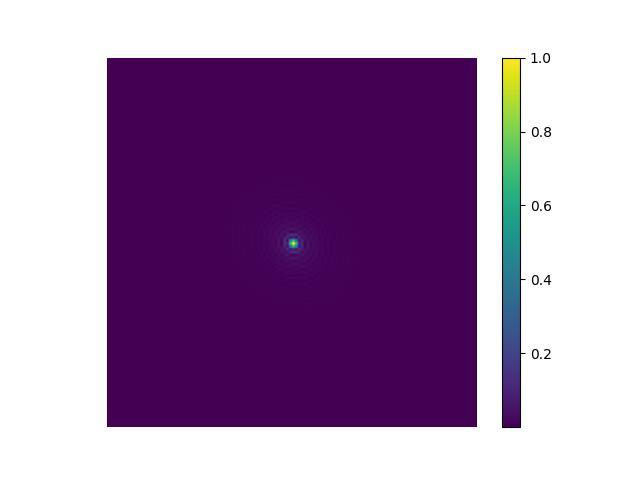
\includegraphics[width=\linewidth]{fig/ft/ft.jpg}
		\caption{The fourier transform of source.}
	\end{subfigure}\hfill
	\begin{subfigure}{0.5\linewidth}
		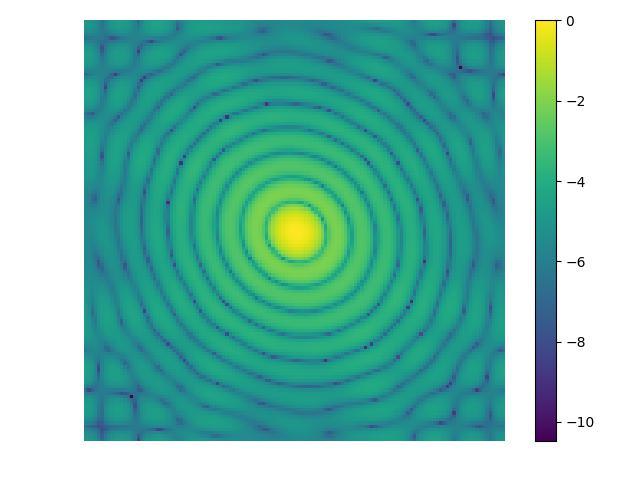
\includegraphics[width=\linewidth]{fig/ft/ft_log.jpg}
		\caption{The logarithmic fourier transform of source.}
	\end{subfigure}
	\caption{Absolute value of the two-dimensional Fast Fourier Transform of fig.~\ref{fig:image} measured by Intensity Interferometry, and observation of maximum (u, v) plane with finite number of baselines can be completed with help of earth's rotation.}
	\label{fig:ft}
\end{figure*}
\begin{figure*}
	\centering
	\begin{subfigure}{0.5\linewidth}
		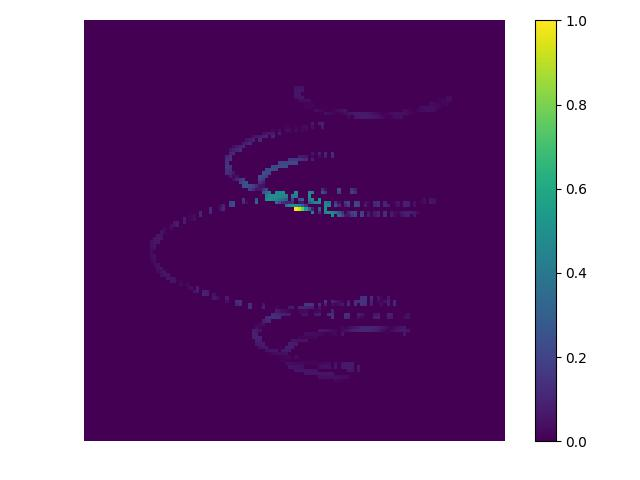
\includegraphics[width=\linewidth]{fig/ft/ft_base.jpg}
		\caption{The fourier transform with baselines.}
	\end{subfigure}\hfill
	\begin{subfigure}{0.5\linewidth}
		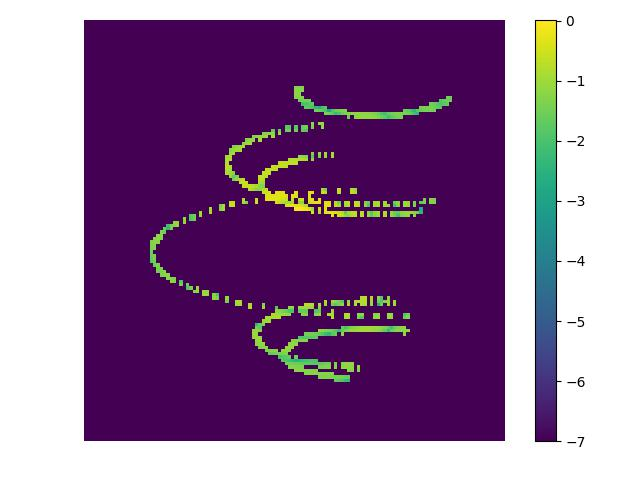
\includegraphics[width=\linewidth]{fig/ft/ft_log_base.jpg}
		\caption{The logarithmic fourier transform with baselines.}
	\end{subfigure}
	\caption{The left panel shows the absolute value of the two-dimensional Fast Fourier Transform of fig.~\ref{fig:image} measured by baselines shown in fig.~\ref{fig:teles}. The right panel shows the same on logarithmic scale}
	\label{fig:ft_base}
\end{figure*}
The primary purpose of IACTs is the study of high energy gamma rays (with energy $E\ \geq 30$ GeV) reaching the Earth from cosmic sources, entering the Earth's atmosphere and seeding the Cherenkov showers in the upper atmosphere due to multiple scattering. These telescopes have an array of mirrors that focus the light onto a set of photo-multiplier tubes (PMTs) \cite{aleksic2016major}. 
\textcolor{blue}{In the simulation model adopted here, a set of four IACTs with similar properties each are considered. The positional configuration of these IACTs is shown in fig.~\ref{fig:teles}. The optical signal guided into a PMT is filtered using a spectral filter with chosen mean observational wavelength $\lambda$ and corresponding bandpass $\Delta \lambda$. 
Use of filters helps in not only reducing back ground noise, but in improving the signal quality and the efficiency of the PMTs also. Filtering background sky light becomes even more significant in II observations as these observations are carried out around full moon nights. Needless to mention that light of the stellar source is focused on the PMT during the II observations.} 
\st{In II observations, the light of a stellar source is focused on a single PMT, which has a filter in front. The purpose of this filter is to efficiently transmit light around mean observational frequency, which protects the PMTs from excessive light. It is necessary, as II observations are mainly done during full moon nights, where it is too bright for Very High Energy $\gamma$-ray observations.} The optical signal of the PMTs is transmitted through optical fibers, converted to an electrical signal, and digitized \cite{acciari2020optical}. The measurable observable is the Pearson's correlation coefficient:
\begin{equation}
	\rho(\tau) = \frac{\left\langle \left( I_1(t) - \left\langle I_1 \right\rangle \right) \cdot \left( I_2(t + \tau) - \left\langle I_2 \right\rangle \right) \right\rangle}{\sqrt{\langle \left( I_1(t) - \langle I_1 \rangle \right)^2 \rangle} \cdot \sqrt{\langle \left( I_2(t) - \langle I_2 \rangle \right) ^2 \rangle}}
	\label{eqn:pearson}
\end{equation}
Since $I_1$ and $I_2$ are proportional to the direct current of the PMTs ($DC_i$), the normalized contrast can be calculated as in equation \ref{eq:norm_contrast2}. One must also correct for a non-constant gain of the PMTs, as well as the moon. The latter can be done by measuring the background light with an additional PMT with no mirrors focused on it \cite{acciari2020optical}. 
\begin{equation}
	c \propto \frac{\rho}{\sqrt{\left(DC_1 \cdot DC_2 \right)}}
	\label{eq:norm_contrast2}
\end{equation}
It must be noted that the calculation of Pearson's correlation coefficient is non-trivial: MAGIC makes use of the convolution theorem for discrete Fourier transforms because it is computationally more efficient.

The significance of the signal can be expressed as the signal-to-noise ratio (SNR), which depends on many factors. However, most importantly, it is proportional to the absolute value of visibility, which itself depends on the distance between the telescopes, shown in equation (\ref{eq:SNR}) \cite{acciari2020optical}.  
\begin{equation}
	SNR = A \cdot \alpha \cdot q \cdot n \cdot \abs{V_{12}}^{2}(d) \cdot \sqrt{b_v} \cdot F^{-1} \cdot \sqrt{\frac{T}{2}} \cdot \sigma
	\label{eq:SNR}
\end{equation}
here, $A$ is the total mirror area, $\alpha$ the quantum efficiency of the PMTs, $q$ the quantum efficiency of the optics, $n$ the differential photon flux from the source, and $b_v$ the cross-correlation bandwidth. The noise of the PMTs is accounted for with $F$, $T$ denotes the observation time, and $\sigma$ is the normalized spectral distribution of the light (including filters) \cite{acciari2020optical}. While most of the parameters can be optimized with hardware, the only way to obtain a better SNR is to increase the observation time with fixed telescopes.  
\textcolor{red}{Points to be discussed: 
\begin{itemize}
\item{Should/Can the final expression for SNR in eq.(\ref{eq:SNR}) be written in terms of $\rho(\tau)$ of eq.(\ref{eqn:pearson}) or $c$ (\ref{eq:norm_contrast2}) in stead of $\vert V_{12}\vert^2$?}
\item{It would be better to generalize the eq.(\ref{eq:norm_contrast2}) to include the signals from all the baseline pairs.}
\end{itemize}}
\subsection{Baseline considerations}
The measurement of the size of stellar objects through absolute visibility depends on the distance between the telescopes, which is called the baseline $d$. 
\begin{equation}
	V_{12}(d) = \frac{c(d)}{c(0)}
	\label{eq:angular_size_meas}
\end{equation}
\textcolor{blue}{For achieving a good SNR with a given telescope configuration, the largest possible observational plane that can be covered is always desirable \citep{acciari2020optical, abeysekara2020demonstration}.}
\begin{comment}
{\st{However, this work needs a good SNR value for high precision of measurement, so the large covered observational plane with telescopes is a necessity for II \citep{acciari2020optical, abeysekara2020demonstration}.} }
\end{comment}
If the source is at the zenith, the coordinates in the Fourier plane ($u,v$) are given by:
\begin{equation}
	(u,v) = \frac{1}{\lambda} (d_N, d_E)
\end{equation}
where $d_N$ and $d_E$ are the baselines expressed in north and east coordinates. 
\textcolor{blue}{But not all sources are at the zenith, and the telescopes are stationary and may also have different relative altitudes $d_A$ depending on the available terrain. Therefore, the Earth's rotation needs to be factored in for covering the maximum observational plane through the rotated baselines. 
For a given stellar source with declination $\delta$, hour-angle $h$ observed by telescopes at latitude $l$, equation (\ref{eq:baseline_rot}) provides the rotated
baselines for a given pair of telescopes \citep{dravins2013optical, saha2020theory}
\begin{equation}
\begin{pmatrix} u\\ v\\ w\\ \end{pmatrix} = R_x(\delta) \cdot R_y(h) \cdot R_x(-l) \begin{pmatrix} d_N\\ d_E\\ d_A\\ \end{pmatrix}
	\label{eq:baseline_rot}
\end{equation}
}
%\end{comment}
\begin{comment}
\st{
Equation (\ref{eq:baseline_rot}), which traces an ellipse for every pair of telescopes. Furthermore, the different altitudes $B_A$ of the telescopes must be considered \cite{dravins2013optical, saha2020theory}.  
\begin{equation}
	\begin{pmatrix} u\\ v\\ w\\ \end{pmatrix} = R_x(\delta) \cdot R_y(h) \cdot R_x(-l) \begin{pmatrix} d_N\\ d_E\\ d_A\\ \end{pmatrix}
	\label{eq:baseline_rot}
\end{equation}
here, $\delta$ is the declination and $h$ is the hour angle of the stellar source, and $l$ is the latitude of the telescopes.}
\end{comment}
The three rotation matrices $R_i$ correspond to the fundamental representation of the SO(3) group \cite{saha2020theory}. Fig.~\ref{fig:base} shows the track of six baselines generated from the telescopes (fig.~\ref{fig:teles}) due to Earth's rotation. Since every pair of telescopes traces an ellipse in the Fourier plane, the total number of ellipses scales as follows:
\begin{equation}
	\label{eq:N_telescopes}
	\mathcal{N} = \frac{N_T \cdot (N_T -1)}{2}
\end{equation}
where $N_T$ is the number of telescopes considered.
As the number of baselines increases non-linearly, II benefits greatly from a large number of telescopes. The planned Cherenkov Telescope Array (CTA) will cover the maximum observational plane and provide insight into stellar objects with optical wavelengths in the future.

\subsection{An Object: Fast Rotating Stars}
In our work presented here, we simulate a single fast-rotating star to test image reconstruction using a GAN. Fast rotation causes stars to take on an oblate shape, flattening at the poles and bulging at the equator due to the existence of stronger centrifugal force \cite{von1924radiative, 1999A&A...347..185M}. Fig.~\ref{fig:image} shows one of the simulations of such a fast-rotating star, \st{where the star takes on an elliptical shape} with brightness distributed across its surface. The brightness is at its maximum at the poles and minimum at the equator, a phenomenon known as gravity darkening \cite{lucy1967gravity}. This effect has been observed first through the interferometric and spectroscopic data from the CHARA Array for the fast-rotating star Regulus \cite{mcalister2005first}. Fast-rotating stars are crucial for understanding various astrophysical processes, including stellar evolution, structure, and \textcolor{red}{dynamics(??? Can we be more elaborate here?)} over time.

Intensity Interferometry measures/counts photons arriving at the telescopes from the stellar object. The correlation of these photon arrivals at the telescopes results in squared visibility (explained in subsection.\ref{sec:signal}). According to Van Cittert Zernike's theorem, this signal is the Fourier transform of brightness distribution in the sky. Fig.~\ref {fig:ft} shows represents the Fourier Transform of the source shown in fig.~\ref{fig:image} using II on linear and logarithmic scale. 
\sout
{However, we do not have an existing technique to observe the complete signals, and we could capture some parts of it only with a one-night simulation, which has been shown in fig.~\ref{fig:ft_base}. It is the covered observational plane using the baselines shown in fig.~\ref{fig:teles}. However, the upcoming CTA promises to cover the maximum observational plane for stellar objects.}
\textcolor{blue}{In order to observe a real stellar source in the sky, however, we would need to receive photons from each point on the surface of the source. This would require infinite number of baselines observing the source over a long enough duration. This demand is obviously not feasible. We have finite number of baselines corresponding to the finite number $N_T$ of telescopes at our disposal and finitely budgeted observation schedule. Therefore, as a pilot, what we have attempted in this work is to simulate the II observation of a sky source over one night duration. Using this finite amount of signal of one night's observation, we have attempted to train a Generative Adversarial Network (GAN) to construct the image of the source.}  

\textcolor{red}{My comments: Suppose we do more simulations with say 8 and 16 telescopes covering the effective ground area, but obviously with 28 and 120 baselines respectively. We can then, perhaps, evolve/suggest some kind of measure (or scale) of quality in resultant image reconstruction with number of telescopes. May be some form of ratios of the SNRs would provide a good comparison. {\bf How much more computationally expensive would it become?}}